%%%%%%%%%%%%%%%%%%%%%%%%%%%%%%%%%%%%%%%%%%%%%%%%%%%%%%%%%%%

% report.tex - 電気情報関係学会 論文
% lualatexでコンパイル

%%%%%%%%%%%%%%%%%%%%%%%%%%%%%%%%%%%%%%%%%%%%%%%%%%%%%%%%%%%

\documentclass[lualatex, twocolumn]{ltjsarticle}

\usepackage{amsmath}
\usepackage{graphicx}
\usepackage{cite}
\usepackage{url}


\title{{\bfseries 環境センシングシステムにおけるIoTデバイスのLoRa通信実機実験に基づいた消費エネルギー評価}\\
\large{Experimental Evaluation of Energy Consumption for a LoRa-based IoT Environmental Sensing System}}
\author{
    河嶋 太陽\textsuperscript{1},
    筒井 弘\textsuperscript{2},
    大鐘 武雄\textsuperscript{2}
    \\
    \normalsize
    Taiyoh Kawashima\textsuperscript{1},
    Hiroshi Tsutsui\textsuperscript{2},
    Takeo Ohgane\textsuperscript{2}
    \\
    \textsuperscript{1}北海道大学工学部,
    \textsuperscript{2}北海道大学大学院情報科学研究院
    \\
    \normalsize
    \textsuperscript{1}School of Engineering/ \textsuperscript{2}Faculty of Information Science and Technology, Hokkaido University
}

\date{}

\begin{document}


\maketitle


\section{はじめに}
 IoT(Internet of things)システムの普及に伴い, 様々な場所でセンシングしたデータを無線通信により収集・記録する機会が増加している. 
多くのIoTデバイスはバッテリーで駆動するため, その通信方式には極めて低い消費電力が要求される. 
この要求に応える技術として,  低消費電力長距離無線通信の一種であるLoRaが注目されている. 
しかし, LoRaが低消費電力であると広く認識されている一方で, その具体的な消費エネルギーの内訳や動作状態を考慮した詳細な分析に関する研究は多くない. 
そこで本稿では,  実際のIoTデバイスとLoRa通信モジュールを用いた測定に基づき, 環境センシングシステムの消費エネルギーの評価を行った. 


\section{環境センシングシステム}
 本研究で構築した環境センシングシステムの構成を図に示す. システムは主に以下の3つのコンポーネントから構成される.
\begin{enumerate}
    \item[(1)]\textbf{IoTデバイス}

    Arduino Nano 33 BLE Sense Rev2を採用した. このボードは内蔵センサにより温度, 湿度, 気圧の測定が可能であるほか, 
    適切にレジスタ操作を行うことによりプロセッサを低消費電力なスリープモードへ移行させる機能を備えている.

    \item[(2)]\textbf{LoRa通信モジュール}

    Ebyte社のE220-900T22Sを用いた. このモジュールは, ArduinoプロセッサからUART通信を介して制御する. 
    また, このモジュール自体も特定の制御ピンの電位を切り替えることでスリープモードへ移行させることができる. 

    \item[(3)]\textbf{電源}

    システムの電源には, 容量110mAhのリチウムポリマーバッテリーを使用し, 各コンポーネントへ給電する.
    なお, 本測定ではバッテリーが尽きるまでの時間を記録するため, 意図的に容量の小さいバッテリーを選択することで測定時間の短縮を図った.

    \item [(4)]\textbf{システムの基本動作}

    本システムの基本的な動作は, Arduino Nano が内蔵センサを用いて温度, 湿度, 気圧を測定し, 取得したデータを
    LoRa通信モジュールを介して送信するというものである. 
    以降の実験は, この一連の動作を一定間隔で繰り返すことにより行う. 
\end{enumerate}


\section{実機実験}
本実験では, 満充電したバッテリーを用いて, 送信開始から送信が途切れるまでの時間を稼働時間とし,
動作間隔を変化させたときの稼働時間を記録した. 
その際に, 各コンポーネントのスリープ機能の導入がシステムの消費エネルギーに与える影響を定量的に評価するために,
(1)スリープ機能を使用しない, (2)LoRa通信モジュールのみスリープ機能を使用する, (3)LoRa通信モジュールとIoTデバイス両方のスリープ機能を使用する, の3つの条件下でそれぞれ同様の実験を行った.

\section{結果と考察}
 3つの測定パターンで得られた、動作間隔と稼働時間の結果を示す前に、
実験結果を分析するためにシステムの総消費エネルギー$E_{\mathrm{total}}$をモデル化する. 
$E_{\mathrm{total}}$は, 1回の動作(センシングと送信)で消費される動的エネルギー$E_{\mathrm{dynamic}}$と, 
待機中に消費される静的エネルギー$P_{\mathrm{static}}\cdot T_{\mathrm{life}}$の和で表される.
稼働時間を$T_{\mathrm{life}}$, 動作間隔を$T_{\mathrm{interval}}$とすると, 動作回数は$T_{\mathrm{life}}/T_{\mathrm{interval}}$となるため, 総エネルギーは次式で定量化される. 
\begin{equation}
    E_{\mathrm{total}} = E_{{\mathrm{dynamic}}} \cdot \frac{T_{\mathrm{life}}}{T_{\mathrm{interval}}} + P_{\mathrm{static}} \cdot T_{\mathrm{life}}
    \label{eq:total_energy}
\end{equation}

バッテリーの総エネルギー$E_{\mathrm{total}}$は一定であると仮定し、式(\ref{eq:total_energy})の両辺を$T_{\mathrm{life}}$で割ると、次式が導出される。
\begin{equation}
  \frac{E_{\mathrm{total}}}{T_{\mathrm{life}}} = E_{\mathrm{dynamic}} \cdot \frac{1}{T_{\mathrm{interval}}} + {P_{\mathrm{static}}}
  \label{eq:linear_model}
\end{equation}

式(\ref{eq:linear_model})は、$y = 1/T_{\mathrm{life}}$、$x = 1/T_{\mathrm{interval}}$と置くと、$y=mx+c$の形式を持つ線形モデルと見なせる。
したがって、実験で得られた稼働時間$T_{\mathrm{life}}$と動作間隔$T_{\mathrm{interval}}$の逆数をプロットし、線形回帰分析を行うことで、
傾き$m=E_{\mathrm{dynamic}}$と切片$c=P_{\mathrm{static}}$をそれぞれ算出できる。
図\ref{fig:results_and_analysis}に, 各測定パターンにおける実測値のプロットと, 上記の線形回帰分析の結果を示す. 

% --- 実験結果と分析結果の図 ---
\begin{figure}[t]
    \centering
    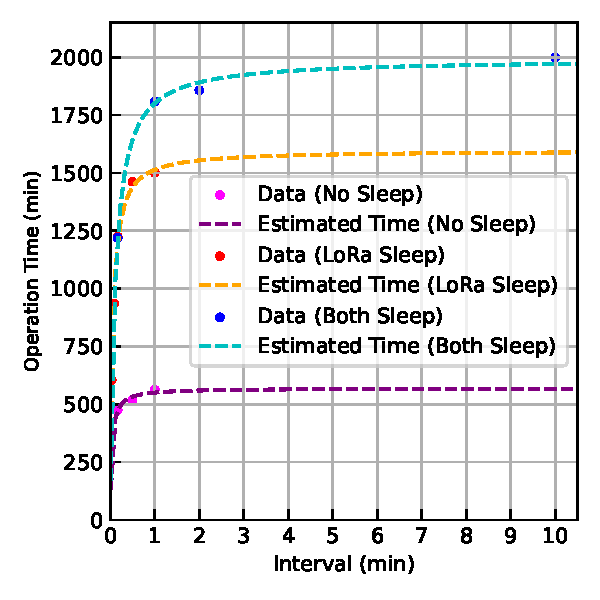
\includegraphics[width=0.9\columnwidth]{figs/Comparison_3patterns.pdf}
    \caption{各測定パターンにおける実験結果と線形回帰分析}
    \label{fig:results_and_analysis}
\end{figure}

\section{まとめ}

\end{document}